\subsubsubsubsection{Sidewalk lane}
\begin{figure}[h]
\centering
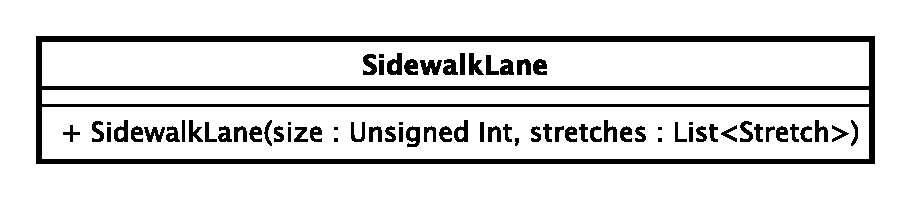
\includegraphics[scale=0.6,keepaspectratio]{images/solution/app/backend/sidewalk_lane.eps}
\caption{\pReactiveComponentLane::SidewalkLane}
\label{fig:sd-app-sidewalk_lane}
\end{figure}
\FloatBarrier
\begin{itemize}
  \item \textbf{\descr} \\
    It represents a sidewalk lane entity. It is a protected object composed of
    one or more (concrete) sidewalk stretches. Only pedestrians can tread this
    kind of lane.
  \item \textbf{\ops}
  \begin{itemize}
  \item[+] \texttt{SidewalkLane(size : Unsigned Int, stretches : List<Stretch>)} \\
  Creates a \texttt{SidewalkLane} object with a specific size and list of stretches.
  \end{itemize}
\end{itemize}
